% !TEX program = pdflatex
% ============================================================
%  BEYOND THE HYPE: A Technical Tour of Quantum Computing Myths
%  Compile with \NOTESMODEtrue for presenter version (notes visible)
%  Compile with \NOTESMODEfalse (default) for audience version
% ============================================================
\documentclass[aspectratio=169,11pt]{beamer}

% ---------- toggle for notes ----------
\newif\ifNOTESMODE
\ifdefined\FORCENOTES
  \NOTESMODEtrue
\else
  \NOTESMODEfalse
\fi

\ifNOTESMODE
  \setbeameroption{show notes on second screen=right}
\else
  \setbeameroption{hide notes}
\fi

% ---------- packages ----------
\usetheme{metropolis}
\usepackage[utf8]{inputenc}
\usepackage{tikz}
\usepackage{pgfplots}
\pgfplotsset{compat=1.17}
\usetikzlibrary{arrows.meta,positioning,shapes,decorations.pathreplacing,calc,fit,backgrounds}
\usepackage{quantikz}
\usepackage{amsmath,amssymb}
\usepackage{booktabs}
\usepackage{array}
\usepackage{textcomp}

% ---------- color palette (quantum theme: deep indigo + cyan) ----------
\definecolor{qIndigo}{HTML}{1B1E3D}
\definecolor{qViolet}{HTML}{4B2E83}
\definecolor{qCyan}{HTML}{00D4C4}
\definecolor{qAmber}{HTML}{FFB020}
\definecolor{qGray}{HTML}{6B7280}
\definecolor{qRed}{HTML}{E4572E}

\setbeamercolor{palette primary}{bg=qIndigo,fg=white}
\setbeamercolor{frametitle}{bg=qIndigo,fg=white}
\setbeamercolor{progress bar}{fg=qCyan,bg=qGray!30}
\setbeamercolor{alerted text}{fg=qRed}
\setbeamercolor{normal text}{fg=qIndigo}
\setbeamercolor{title separator}{fg=qCyan}
\setbeamertemplate{itemize items}[circle]
\setbeamercolor{itemize item}{fg=qCyan}
\setbeamercolor{itemize subitem}{fg=qViolet}

\newcommand{\myth}[1]{\textbf{\alert{MYTH:}} #1}
\renewcommand{\fact}[1]{\textbf{\textcolor{qCyan!70!black}{FACT:}} #1}
\newcommand{\predictlabel}{\textbf{\textcolor{qAmber!80!black}{QUICK PREDICTION:}}}
\newcommand{\soundstruelabel}{\textbf{\textcolor{qViolet}{Why this sounds true:}}}
\newcommand{\actuallylabel}{\textbf{\textcolor{qRed}{Where it breaks down:}}}

\title{Beyond the Hype}
\subtitle{A Technical Tour of Quantum Computing Myths}
\author{}
\date{}

% ============================================================
%  REUSABLE TIKZ DIAGRAMS
% ============================================================

% ---- Bloch-sphere-style qubit diagram ----
\newcommand{\blochdiagram}[1][35]{
\begin{tikzpicture}[scale=1.15]
  \draw[qGray, thick] (0,0) circle (2);
  \draw[qGray] (0,2) ellipse (2 and 0.55);
  \draw[qGray!70, dashed] (-2,0) arc (180:360:2 and 0.55);
  \draw[qGray!70] (-2,0) arc (180:0:2 and 0.55);
  \draw[qIndigo, -{Latex[length=2.5mm]}] (0,0) -- (0,2.3) node[above]{$|0\rangle$};
  \draw[qIndigo, -{Latex[length=2.5mm]}] (0,0) -- (0,-2.3) node[below]{$|1\rangle$};
  \draw[qViolet, -{Latex[length=2.5mm]}, very thick]
       (0,0) -- ({2*sin(#1)},{2*cos(#1)}) node[right,xshift=1mm]{$|\psi\rangle$};
  \draw[qGray, densely dotted] (0,0) -- ({2*sin(#1)},0);
  \node[qGray, below] at ({sin(#1)},0) {\scriptsize $\sin(\theta/2)$};
\end{tikzpicture}
}

% ---- Hardware modality icon row ----
\newcommand{\hwicons}{
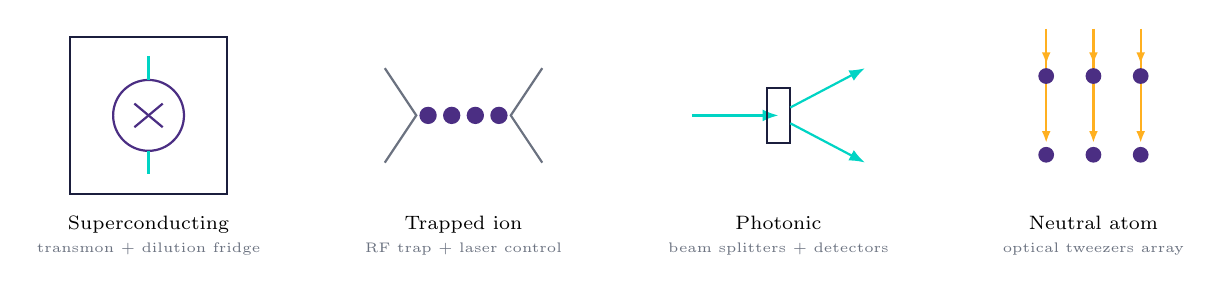
\begin{tikzpicture}[scale=1]
  % ---- Superconducting ----
  \begin{scope}[shift={(0,0)}]
    \draw[qIndigo,thick] (-1,-1) rectangle (1,1);
    \draw[qViolet,thick] (0,0) circle(0.45);
    \draw[qViolet,thick] (-0.18,0.15)--(0.18,-0.15);
    \draw[qViolet,thick] (-0.18,-0.15)--(0.18,0.15);
    \draw[qCyan,thick] (0,0.45)--(0,0.75);
    \draw[qCyan,thick] (0,-0.45)--(0,-0.75);
    \node[below] at (0,-1.15) {\scriptsize Superconducting};
    \node[below,qGray] at (0,-1.5) {\tiny transmon $+$ dilution fridge};
  \end{scope}
  % ---- Trapped ion ----
  \begin{scope}[shift={(4,0)}]
    \draw[qGray,thick] (-1,0.6) -- (-0.6,0) -- (-1,-0.6);
    \draw[qGray,thick] (1,0.6) -- (0.6,0) -- (1,-0.6);
    \foreach \x in {-0.45,-0.15,0.15,0.45}{
      \fill[qViolet] (\x,0) circle (0.11);
    }
    \node[below] at (0,-1.15) {\scriptsize Trapped ion};
    \node[below,qGray] at (0,-1.5) {\tiny RF trap $+$ laser control};
  \end{scope}
  % ---- Photonic ----
  \begin{scope}[shift={(8,0)}]
    \draw[qCyan,thick,-{Latex[length=2mm]}] (-1.1,0) -- (0,0);
    \draw[qIndigo,thick] (-0.15,-0.35) rectangle (0.15,0.35);
    \draw[qCyan,thick,-{Latex[length=2mm]}] (0.15,0.1) -- (1.1,0.6);
    \draw[qCyan,thick,-{Latex[length=2mm]}] (0.15,-0.1) -- (1.1,-0.6);
    \node[below] at (0,-1.15) {\scriptsize Photonic};
    \node[below,qGray] at (0,-1.5) {\tiny beam splitters $+$ detectors};
  \end{scope}
  % ---- Neutral atom ----
  \begin{scope}[shift={(12,0)}]
    \foreach \x in {-0.6,0,0.6}{
      \foreach \y in {-0.5,0.5}{
        \draw[qAmber,thick,-{Latex[length=1.5mm]}] (\x,1.1) -- (\x,\y+0.15);
        \fill[qViolet] (\x,\y) circle (0.1);
      }
    }
    \node[below] at (0,-1.15) {\scriptsize Neutral atom};
    \node[below,qGray] at (0,-1.5) {\tiny optical tweezers array};
  \end{scope}
\end{tikzpicture}
}

% ---- Milestone timeline ----
\newcommand{\timeline}{
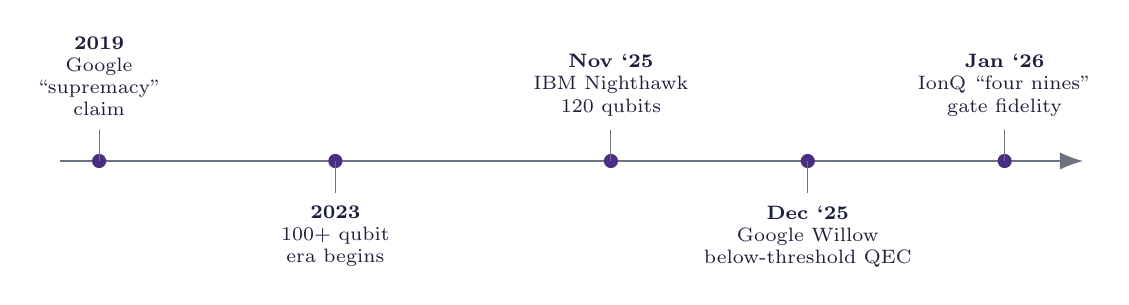
\begin{tikzpicture}[scale=1]
  \draw[qGray, thick,-{Latex[length=3mm]}] (0,0) -- (13,0);
  \foreach \x/\lbl/\txt in {
     0.5/2019/{Google\\``supremacy''\\claim},
     7/{Nov `25}/{IBM Nighthawk\\120 qubits},
     12/{Jan `26}/{IonQ ``four nines''\\gate fidelity}}{
     \fill[qViolet] (\x,0) circle(0.09);
     \draw[qGray] (\x,0) -- (\x,0.4);
     \node[align=center, font=\scriptsize, qIndigo, anchor=south] at (\x,0.45) {\textbf{\lbl}\\\txt};
  }
  \foreach \x/\lbl/\txt in {
     3.5/2023/{100+ qubit\\era begins},
     9.5/{Dec `25}/{Google Willow\\below-threshold QEC}}{
     \fill[qViolet] (\x,0) circle(0.09);
     \draw[qGray] (\x,0) -- (\x,-0.4);
     \node[align=center, font=\scriptsize, qIndigo, anchor=north] at (\x,-0.45) {\textbf{\lbl}\\\txt};
  }
\end{tikzpicture}
}

% ---- Surface-code style patch ----
\newcommand{\surfacecode}{
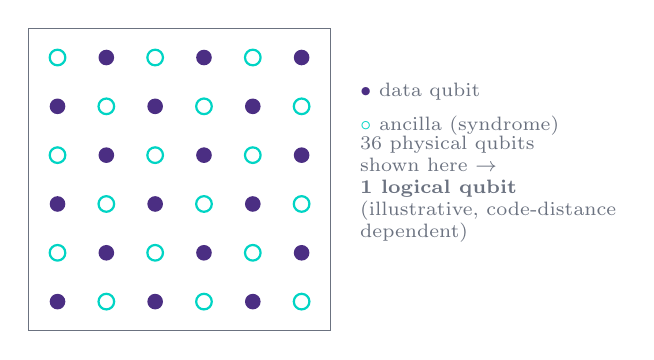
\begin{tikzpicture}[scale=0.62]
  \foreach \x in {0,...,5}{
    \foreach \y in {0,...,5}{
      \ifodd\numexpr\x+\y\relax
        \draw[qCyan,thick] (\x,\y) circle(0.16);
      \else
        \fill[qViolet] (\x,\y) circle(0.16);
      \fi
    }
  }
  \draw[qGray,thin] (-0.6,-0.6) rectangle (5.6,5.6);
  \node[qGray, anchor=west, font=\scriptsize] at (6,4.3) {\textcolor{qViolet}{$\bullet$} data qubit};
  \node[qGray, anchor=west, font=\scriptsize] at (6,3.6) {\textcolor{qCyan}{$\circ$} ancilla (syndrome)};
  \node[qGray, anchor=west, font=\scriptsize,align=left] at (6,2.3)
      {36 physical qubits\\shown here $\rightarrow$\\ \textbf{1 logical qubit}\\(illustrative, code-distance\\dependent)};
\end{tikzpicture}
}

% ---- Complexity class map ----
\newcommand{\complexitymap}{
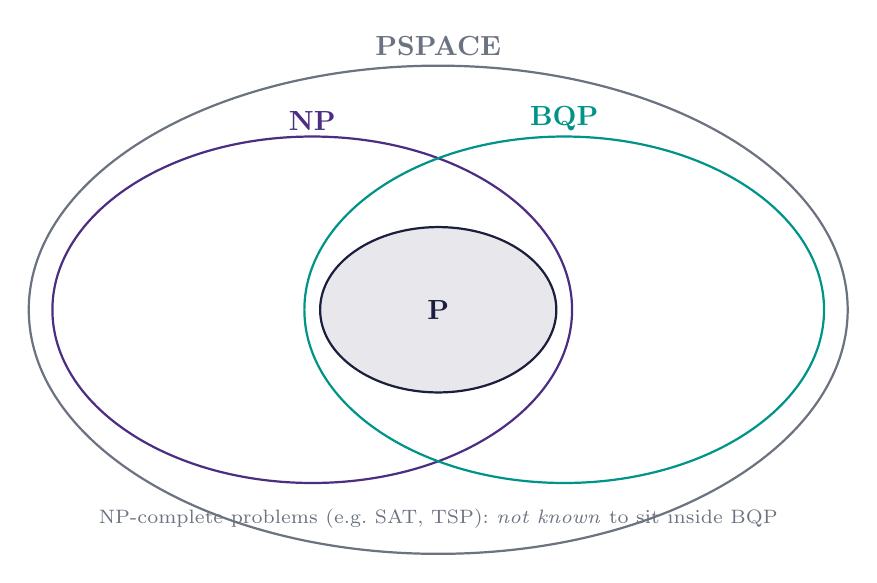
\begin{tikzpicture}[scale=1]
  \draw[qGray, thick] (0,0) ellipse (5.2 and 3.1);
  \node[qGray, above] at (0,3.1) {\textbf{PSPACE}};
  \draw[qViolet, thick] (-1.6,0) ellipse (3.3 and 2.2);
  \node[qViolet, above] at (-1.6,2.15) {\textbf{NP}};
  \draw[qCyan!70!black, thick] (1.6,0) ellipse (3.3 and 2.2);
  \node[qCyan!70!black, above] at (1.6,2.15) {\textbf{BQP}};
  \draw[qIndigo, thick, fill=qIndigo!10] (0,0) ellipse (1.5 and 1.05);
  \node[qIndigo] at (0,0) {\textbf{P}};
  \node[qGray, align=left, font=\scriptsize] at (0,-2.65)
     {NP-complete problems (e.g.\ SAT, TSP): \emph{not known} to sit inside BQP};
\end{tikzpicture}
}

\begin{document}

% ============================================================
\begin{frame}[plain]
  \titlepage
  \note{
    Welcome. Open with energy, not apology. This talk has two audiences in the
    room today: administrators deciding on curriculum, and students deciding
    whether to care. Promise both: (1) I will debunk the hype, (2) I will show
    you the real, still-remarkable science underneath, and (3) I will make the
    case, with data, for why this belongs in our curriculum NOW, not in five years.
    Keep opening under 2 minutes.
  }
\end{frame}

% ============================================================
\begin{frame}{Pop quiz -- raise your hand}
  \begin{center}
  \Large Which of these is \textbf{true}?
  \end{center}
  \vspace{2mm}
  \begin{enumerate}
    \item Quantum computers try every possible answer simultaneously
    \item Quantum computers can already break Bitcoin / all encryption
    \item Quantum computers will replace classical computers
    \item \textbf{None of the above}
  \end{enumerate}
  \vspace{3mm}
  \begin{center}
  \textcolor{qGray}{\emph{(Take a moment. Raise your hand for the one you believe.)}}
  \end{center}
  \note{
    Actually pause here and get hands up for each of the four options --
    don't skip this, it's the single highest-leverage moment in the talk.
    Whatever the vote splits like, say: "Interesting -- by the end of this
    talk you'll be able to explain, technically, why the correct answer is
    (4), and exactly what's half-true about the other three." This turns
    the entire rest of the talk into a payoff the audience is owed, rather
    than a lecture they're receiving. Do not reveal the answer yet. If the
    room is shy, self-report you would have voted for one of them before
    you learned the details -- lowers the stakes of guessing wrong.
  }
\end{frame}

% ============================================================
\begin{frame}{Why this talk exists}
  \begin{itemize}
    \item Quantum computing: one of the most \alert{hyped} \emph{and}
          most \alert{misunderstood} topics in computer science today
    \item My claim: \textbf{all four options on the last slide are wrong
          as literally stated} --- but each is built on a real, technical
          truth underneath
    \item Format: \textbf{Myth} $\rightarrow$ \textbf{Fact}, taken apart
          technically, explained so \emph{everyone} in the room follows it
  \end{itemize}
  \note{
    Keep this very short -- 60-90 seconds -- since the pop quiz already did
    the job of setting stakes. Land the phrase "built on a real truth
    underneath" -- it previews the "why this sounds true / where it breaks
    down" pattern you'll repeat through the talk. Consider asking a show
    of hands: who has used Qiskit / IBM Quantum Experience? Use the answer
    to calibrate how much hand-holding the linear-algebra parts need.
  }
\end{frame}

% ============================================================
\begin{frame}{Roadmap}
  \begin{enumerate}
    \item What \emph{is} a qubit, really? (5 min)
    \item Myths about \textbf{existence \& hardware} (15 min)
    \item Myths about \textbf{what quantum computers can do} (20 min)
    \item Myths about \textbf{the physics} --- parallelism, entanglement (20 min)
    \item Myths about \textbf{cryptography} (10 min)
    \item Putting it together, then \textbf{why this matters for us} (15 min)
    \item Curriculum sketch, resources, Q\&A (10 min)
  \end{enumerate}
  \note{
    Roughly 95-100 minutes total as outlined; trim section 3 or 4 if running
    at the 60-minute end, expand Q\&A and section 6 if the audience skews
    administration-heavy. Section 6 is the payload for the deans in the room
    -- do not let it get squeezed by running long earlier. Remind the room
    we'll return to the pop quiz at the very end.
  }
\end{frame}

% ============================================================
\section{What is a Qubit, Really?}

\begin{frame}{From bit to qubit}
  \begin{columns}
    \begin{column}{0.48\textwidth}
      \textbf{Classical bit}
      \begin{itemize}
        \item State: $0$ \emph{or} $1$
        \item Read any time, no disturbance
      \end{itemize}
    \end{column}
    \begin{column}{0.48\textwidth}
      \textbf{Qubit}
      \begin{itemize}
        \item State: $|\psi\rangle=\alpha|0\rangle+\beta|1\rangle$
        \item $\alpha,\beta \in \mathbb{C}$, $|\alpha|^2+|\beta|^2=1$
        \item Measuring \emph{forces} a choice: $0$ w.p. $|\alpha|^2$, $1$ w.p.\ $|\beta|^2$
      \end{itemize}
    \end{column}
  \end{columns}
  \vspace{2mm}
  \begin{alertblock}{The one idea to hold onto all talk}
    A qubit is not ``0 and 1 at once.'' It is a \textbf{vector of complex
    amplitudes} that determines probabilities --- and those amplitudes can
    \textbf{interfere}, constructively or destructively. That interference is
    the entire engine of quantum computing.
  \end{alertblock}
  \note{
    This slide is the foundation for every later myth-debunk. Spend real
    time here even though it looks short. Write $\alpha|0\rangle + \beta|1\rangle$
    on the board if you have one. Emphasize: amplitude is not probability --
    amplitudes are complex numbers, can be negative or have phase, and
    PROBABILITY is the squared magnitude. This is exactly why interference
    (cancellation) is possible -- a concept impossible to state in classical
    probability. Preview: myth about ``testing every answer at once by magic''
    will come back to this slide directly.
  }
\end{frame}

\begin{frame}{Superposition, geometrically}
  \begin{columns}
    \begin{column}{0.55\textwidth}
      \blochdiagram[35]
    \end{column}
    \begin{column}{0.45\textwidth}
      \begin{itemize}
        \item Every pure single-qubit state is a point on this sphere
        \item Poles = $|0\rangle$, $|1\rangle$ (classical bit values)
        \item Everywhere else = genuine superposition
        \item Quantum \textbf{gates} = rotations of this vector
        \item $n$ qubits $\Rightarrow$ state lives in a $2^n$-dimensional
              space --- \emph{that} is the resource, not ``storage''
      \end{itemize}
    \end{column}
  \end{columns}
  \note{
    This is the Bloch sphere. Mention it by name -- students who go on to
    take a quantum course will see this exact picture in week 1. Rotations
    (X, Y, Z, Hadamard gates) move the vector around the sphere. Flag the
    last bullet -- it's a planted seed for the "exponential storage" myth
    later: a $2^n$ dimensional description does NOT mean $2^n$ classical bits
    you can extract, since a single measurement collapses to n classical bits.
  }
\end{frame}

% ============================================================
\section{Myth 1: ``Quantum Computers Don't Really Exist''}

\begin{frame}{\myth{Quantum computers don't exist -- it's vaporware}}
  \fact{Real machines, several competing physical technologies}
  \vspace{3mm}
  \hwicons
  \note{
    Walk through each icon left to right, ~30 seconds each:
    - Superconducting (IBM, Google, Rigetti): artificial atoms made of
      niobium/aluminum circuits, cooled in dilution refrigerators to ~15 mK,
      controlled with microwave pulses. Most mature, most heavily funded.
    - Trapped ion (IonQ, Quantinuum): individual ions held by oscillating
      electric fields (Paul trap), qubit = electronic energy levels (a
      hyperfine or optical transition) -- correct the common "electron orbit"
      misconception explicitly here. Manipulated with laser pulses. Runs at
      room temperature in vacuum, generally the highest gate fidelities.
    - Photonic (Xanadu, PsiQuantum): qubit = properties of single photons
      (e.g. path or polarization), manipulated with beam splitters and phase
      shifters, detected with single-photon detectors. Naturally networkable,
      does not need extreme cooling for the qubits themselves.
    - Neutral atom (QuEra, Pasqal, Atom Computing): individual atoms held in
      place by tightly focused laser beams ("optical tweezers"), arranged in
      programmable arrays, qubit = atomic energy levels, entangled via
      Rydberg-state interactions.
    Emphasize: this is not one lab experiment, it's several billion-dollar
    engineering programs racing in parallel, each with real trade-offs.
  }
\end{frame}

\begin{frame}{Milestones: this moved fast}
  \resizebox{\textwidth}{!}{\timeline}
  \vspace{4mm}
  \begin{itemize}
    \item IBM's 2025 \textbf{Nighthawk} processor: 120 qubits, 218 tunable
          couplers, targeting \emph{verified} quantum advantage by end of 2026
    \item Google's \textbf{Willow} chip: first demonstration of error
          correction that gets \emph{better}, not worse, as you add qubits
          (``below threshold'')
    \item IonQ: two-qubit gate fidelity of \textbf{99.99\%} (``four nines'')
  \end{itemize}
  \note{
    Numbers current as of mid-2026 -- say so explicitly, this field moves
    fast enough that specific figures should be treated as a snapshot, not
    gospel. The Willow "below threshold" result is arguably the single most
    important recent result: it means for the first time that scaling up
    the error-correcting code actually suppresses the logical error rate
    exponentially, rather than accumulating more physical noise than it
    fixes. This is the trend line that makes "myth 2" on the next slide
    non-trivial to explain -- errors are a real limiter, but the curve just
    bent in the right direction for the first time.
  }
\end{frame}

% ============================================================
\section{Myth 2: ``We Already Have Working, Useful Quantum Computers''}

\begin{frame}{\myth{We already have a working quantum computer beating classical machines at real problems}}
  \fact{We're in the \textbf{NISQ} era: Noisy, Intermediate-Scale Quantum}
  \begin{itemize}
    \item Today's devices: $\sim$50--1000+ \textbf{physical} qubits, but
          \emph{noisy} -- gate error rates of order $10^{-3}$
    \item Decoherence: qubits lose their quantum state from stray heat,
          radiation, and fabrication imperfections in microseconds to
          milliseconds
    \item Fix: \textbf{quantum error correction} -- spread \emph{one} reliable
          ``logical'' qubit across \emph{many} noisy physical qubits
  \end{itemize}
  \note{
    "NISQ" is a term coined by John Preskill in 2018 -- worth naming, gives
    students a keyword to search. Contrast with classical computers: a
    classical bit is stable for years; a physical qubit today is stable for
    microseconds to milliseconds. This fragility, not lack of qubits, is the
    actual bottleneck the entire industry is fighting. This directly refutes
    any claim that we're close to "quantum computers doing everything
    classical computers do, but faster" -- we're not yet at reliable
    general-purpose fault-tolerant computation.
  }
\end{frame}

\begin{frame}{Physical qubits vs.\ logical qubits}
  \begin{columns}
    \begin{column}{0.52\textwidth}
      \resizebox{\textwidth}{!}{\surfacecode}
    \end{column}
    \begin{column}{0.48\textwidth}
      \begin{itemize}
        \item \textbf{Surface code} (one popular scheme): encode 1 logical
              qubit across a 2D patch of physical qubits
        \item More physical qubits per patch $\Rightarrow$ exponentially
              lower logical error rate --- \emph{if} physical error rate is
              below a threshold
        \item Estimates for breaking RSA-2048 with Shor's algorithm:
              on the order of \textbf{millions} of physical qubits with
              today's error rates
      \end{itemize}
    \end{column}
  \end{columns}
  \begin{alertblock}{The one line to remember}
    A machine advertised as ``a million qubits'' may still behave, in
    practice, like only a \textbf{few thousand perfect ones}.
  \end{alertblock}
  \note{
    Be careful with the RSA estimate -- state it as an order-of-magnitude
    estimate from the literature (Gidney \& Ekera and follow-up work), not a
    fixed number, since it depends heavily on assumed physical error rates
    and code distance, and has been revised downward over time as algorithms
    improve. The core teaching point: qubit COUNT headlines (120, 1000+) are
    almost all physical qubits, not logical/error-corrected qubits -- that
    distinction alone will inoculate the audience against 90\% of hype
    articles they'll read afterward. Land the alert-block line slowly and
    let it sit for a second before moving on -- it's designed to be the
    one sentence from this slide people still repeat a year later.
  }
\end{frame}

% ============================================================
\section{Myth 3: ``Quantum Computers Will Replace Classical Computers''}

\begin{frame}{\myth{Quantum computers will replace classical computing entirely}}
  \soundstruelabel\ ``It's exponentially more powerful, so it must beat
  classical computers at \emph{everything}.''

  \vspace{2mm}
  \actuallylabel
  \begin{itemize}
    \item Quantum speedups exploit specific \textbf{mathematical structure}
          (periodicity, unstructured search, entanglement in the problem
          itself) -- most everyday computing has none of that structure
    \item \textbf{Sorting, arithmetic, running a browser or a database}:
          no known quantum speedup, and for some (e.g.\ comparison-based
          sorting) speedups are \emph{provably} not going to appear
    \item A classical laptop will keep doing your email forever
  \end{itemize}
  \note{
    This is a myth students especially arrive with, from pop-sci headlines.
    Sorting is a clean example: comparison sort has a proven classical lower
    bound of Omega(n log n) comparisons, and there is no known quantum
    algorithm that beats this asymptotically for general comparison-based
    sorting -- the black-box speedups quantum computers get (like Grover)
    are for UNSTRUCTURED SEARCH, not sorting, and don't transfer. Land the
    point: "quantum computer" is closer to "specialized coprocessor" (like a
    GPU) than "faster general CPU" -- most future systems will be hybrid
    classical+quantum, with the quantum part handling one narrow subroutine.
  }
\end{frame}

\begin{frame}{\predictlabel}
  \Large
  \begin{center}
  Of these four -- \textbf{Shor}, \textbf{Grover}, \textbf{quantum
  simulation}, \textbf{QAOA} -- \\[2mm]
  which ones have a \emph{proven} exponential speedup over the best
  known classical algorithm?
  \end{center}
  \note{
    Let a few people call out guesses before advancing. Answer on the next
    slide: Shor -- yes, proven exponential (for factoring). Quantum
    simulation -- yes, for simulating quantum systems themselves. Grover --
    proven, but only QUADRATIC, not exponential (a common wrong guess).
    QAOA/VQE -- no proof at all, purely empirical heuristic evidence so far
    (the most common wrong guess is that this one is exponential, because
    marketing language rarely distinguishes "quantum-powered" from
    "provably faster"). This pause makes the table on the next slide land
    as a reveal rather than a wall of text.
  }
\end{frame}

\begin{frame}{Where the real speedups live}
  \begin{table}
  \small
  \begin{tabular}{@{}p{2.6cm}p{4.6cm}p{4.4cm}@{}}
    \toprule
    \textbf{Algorithm} & \textbf{What it speeds up} & \textbf{Type of speedup} \\
    \midrule
    Shor (1994) & Integer factoring, discrete log & Exponential \\
    Grover (1996) & Unstructured search over $N$ items & Quadratic ($\sqrt{N}$) \\
    Quantum simulation & Simulating quantum systems (chemistry, materials) & Exponential (for some systems) \\
    QAOA / VQE & Combinatorial \& chemistry optimization (heuristic) & Unproven, problem-dependent \\
    \bottomrule
  \end{tabular}
  \end{table}
  \note{
    Emphasize the honesty of row 4 -- QAOA and VQE are the algorithms behind
    most "quantum for finance / logistics / drug discovery" press releases,
    and they are HEURISTICS: there is no proof of speedup, only empirical
    exploration, similar in spirit to how we use heuristics in classical
    optimization (simulated annealing, genetic algorithms) without a proof
    they beat exact methods in general. This is a good moment to say
    "skepticism of a specific claim is not the same as skepticism of the
    whole field" -- exactly the nuance you want administrators to absorb.
    Quantum simulation (Feynman's original 1981 motivation for the whole
    field) is arguably the most likely first genuinely useful application:
    simulating molecules and materials, which is itself an exponentially
    hard problem for classical computers because quantum systems have
    exponentially many amplitudes to track.
  }
\end{frame}

% ============================================================
\section{Myth 4: ``Quantum Computers Solve P = NP''}

\begin{frame}{\myth{Quantum computers solve P = NP / can crack any hard problem instantly}}
  \fact{Quantum computing has its own complexity class: \textbf{BQP}}
  \centering
  \resizebox{0.75\textwidth}{!}{\complexitymap}
  \note{
    Walk the diagram outward-in: P is what classical computers solve
    efficiently. NP is what can be VERIFIED efficiently (includes P, plus
    much more, including NP-complete problems like SAT and TSP). BQP
    (Bounded-error Quantum Polynomial time) is what quantum computers solve
    efficiently. Known: P is contained in BQP (quantum computers can do
    anything classical computers can). NOT known: whether BQP contains all
    of NP, or whether NP-complete problems are in BQP. Consensus belief among
    complexity theorists: quantum computers do NOT solve NP-complete problems
    in polynomial time -- Grover's algorithm gives a quadratic (root-N), not
    exponential, speedup for brute-force search over NP-complete problems,
    which is a real speedup but does not collapse P vs NP. This directly
    kills the "instantly crack any problem" myth with an actual theorem-level
    argument, not just "trust me."
  }
\end{frame}

\begin{frame}{Grover's algorithm, without equations}
  \begin{center}
  \Large Imagine a maze with $N$ doors, one correct.
  \end{center}
  \vspace{3mm}
  \begin{columns}
    \begin{column}{0.48\textwidth}
      \textbf{Classical search}
      \begin{itemize}
        \item Open door 1, door 2, door 3, \ldots
        \item Worst case: check all $N$ doors
      \end{itemize}
    \end{column}
    \begin{column}{0.48\textwidth}
      \textbf{Grover's search}
      \begin{itemize}
        \item \emph{Not} opening all doors at once
        \item Each round, the \textbf{correct door glows brighter} and
              the wrong ones dim slightly
        \item After $\sim\sqrt{N}$ rounds: open the brightest door
      \end{itemize}
    \end{column}
  \end{columns}
  \note{
    This is the "no equations" intuition pump for Grover -- use it BEFORE
    the circuit diagram on the next slide, then use the circuit for anyone
    who wants the actual mechanism. "Glowing brighter" = constructive
    interference increasing the marked state's amplitude; "dimming" = the
    unmarked states' amplitudes decreasing. Be honest that this is a
    metaphor, not the mechanism, and that the real mechanism (reflections
    about the average amplitude) is on the next slide for those who want it.
    This is a good moment for the "why does the parallelism myth sound
    plausible" comment: it FEELS like checking every door at once because
    every door does get a peek in superposition -- but only the amplitude
    pattern, not a full open-and-check, and only the brightest one survives
    measurement at the end.
  }
\end{frame}

\begin{frame}{What a quadratic speedup actually looks like}
  \centering
  \begin{quantikz}
    \lstick{$|0\rangle^{\otimes n}$} & \gate{H^{\otimes n}} & \gate[2]{\text{Oracle } U_f} & \gate[2]{\text{Diffusion}} & \qw & \meter{} \\
    \lstick{$|{-}\rangle$} & \qw & & & \qw & \qw
  \end{quantikz}
  \vspace{3mm}
  \begin{itemize}
    \item Repeat the Oracle + Diffusion block $\sim \frac{\pi}{4}\sqrt{N}$ times
    \item Classical unstructured search: $O(N)$ tries. Grover: $O(\sqrt{N})$
    \item Real, provable, and still \textbf{not} exponential
  \end{itemize}
  \note{
    This is Grover's algorithm sketch. The oracle marks the answer by
    flipping its phase (phase kickback via the ancilla in the minus state);
    the diffusion operator reflects amplitudes about their average, which
    amplifies the marked state's amplitude a little on each round. After
    about (pi/4) * sqrt(N) rounds, the marked state's probability is close
    to 1. Contrast size: for N = 1 trillion, classical brute force needs
    ~1 trillion tries; Grover needs ~880,000 -- meaningful, but nowhere near
    the exponential blowup people imagine when they hear "cracks any
    problem instantly."
  }
\end{frame}

% ============================================================
\section{Myth 5: ``They Test Every Answer at Once, by Magic''}

\begin{frame}{\myth{Quantum computers try every possible answer simultaneously, ``by magic''}}
  \soundstruelabel\ superposition really does give the machine
  \emph{access} to all $2^n$ basis states at once.

  \vspace{3mm}
  \predictlabel\ if that were the whole story, why doesn't a quantum
  computer solve \textbf{every} NP-complete problem -- Sudoku, TSP,
  scheduling -- \emph{instantly}?

  \note{
    Pause after the prediction question -- let the room sit with the
    contradiction for a few seconds before advancing. This is the
    "detective story" structure: state the plausible-sounding premise,
    then expose the contradiction it implies, THEN resolve it on the next
    slide. Don't answer it yet. If someone shouts an answer, acknowledge
    it but say "hold that thought, exact mechanism next slide."
  }
\end{frame}

\begin{frame}{\actuallylabel\ measurement only reveals one answer}
  \fact{It's \textbf{interference}, not magic -- and it's fragile}
  \begin{itemize}
    \item Superposition gives \emph{access} to all $2^n$ basis states --
          but a single measurement reveals only \textbf{one}, chosen at
          random by the amplitudes
    \item The actual trick: design a circuit so amplitudes leading to
          \textbf{wrong} answers cancel (destructive interference), and
          amplitudes leading to the \textbf{right} answer reinforce
          (constructive interference)
    \item If you don't engineer that interference pattern, superposition
          alone buys you \emph{nothing} -- you'd just measure noise
    \item That engineering is \textbf{hard} and problem-specific --
          which is exactly why Sudoku doesn't fall out for free
  \end{itemize}
  \note{
    This is the most important conceptual correction of the whole talk. The
    popular claim "it checks every answer at once" describes superposition
    but silently ignores measurement collapse -- if that were the whole
    story, EVERY quantum algorithm would instantly solve EVERY problem,
    which is obviously false (see previous section, and the prediction
    question on the last slide). The actual source of power is designing
    constructive/destructive interference so that only the useful answers
    survive to measurement time -- this is genuinely hard algorithm design,
    not a free lunch from parallelism. This is why only a handful of
    quantum algorithms exist after 30 years, despite full access to
    superposition being "free." Tie back explicitly to the Grover
    "glowing door" analogy from the previous section -- same underlying
    mechanism, interference reshaping amplitudes round by round.
  }
\end{frame}

\begin{frame}{A toy example: Deutsch--Jozsa}
  \centering
  \begin{quantikz}
    \lstick{$|0\rangle^{\otimes n}$} & \gate{H^{\otimes n}} & \gate[2]{U_f} & \gate{H^{\otimes n}} & \meter{} & \rstick{\text{constant or balanced?}}\\
    \lstick{$|1\rangle$} & \gate{H} & & \qw & \qw &
  \end{quantikz}
  \begin{itemize}
    \item Question: is a hidden function $f$ \emph{constant} or
          \emph{balanced}? Classically: up to $2^{n-1}+1$ queries
          in the worst case
    \item Quantumly: \textbf{one} query, thanks to interference
          cancelling all ``balanced'' outcomes when $f$ is constant
    \item Toy problem, but historically the first clean proof that
          interference $>$ brute force
  \end{itemize}
  \note{
    Deutsch-Jozsa (1992) is a good toy example because the interference
    argument is small enough to actually walk through the math if you have
    a blackboard/whiteboard and time, but simple enough to just assert here
    if time is short. Key phrase for the audience to retain: quantum
    algorithms don't parallelize the SEARCH, they parallelize the
    QUESTION-ASKING in a way that lets wrong answers cancel. It has no
    direct practical use itself (nobody needs to solve this exact promise
    problem) but it's the historical proof-of-concept that opened the field.
  }
\end{frame}

% ============================================================
\section{Myth 6: ``More Qubits = Exponential Storage''}

\begin{frame}{\myth{$n$ qubits store $2^n$ classical bits of information}}
  \predictlabel\ you measure a 300-qubit chip once. How many classical
  bits do you get out -- $2^{300}$, or something much smaller?

  \vspace{3mm}
  \fact{The $2^n$-dimensional description is a \textbf{computational resource},
        not readable storage}
  \begin{itemize}
    \item Describing an $n$-qubit state on paper does take $2^n$ complex
          numbers -- that's real, and it's why classical computers struggle
          to \emph{simulate} quantum systems
    \item But \textbf{measuring} $n$ qubits yields exactly $n$ classical
          bits, once, and the state collapses -- you cannot read out the
          exponential description
    \item Practical bottleneck is often not qubit \emph{count} but
          \textbf{connectivity, coherence time, and gate fidelity} --- this
          is why benchmarks like \emph{Quantum Volume} or \emph{Algorithmic
          Qubits} matter more than a raw qubit number in vendor marketing
  \end{itemize}
  \note{
    Let someone answer the prediction out loud -- the "obviously correct"
    wrong answer is 2 to the power 300 (a number bigger than atoms in the
    universe); the right answer is exactly 300 classical bits, once, per
    shot. This
    myth comes from confusing the size of the MATHEMATICAL DESCRIPTION
    of a quantum state (which genuinely is exponential -- this is why
    classical simulation of quantum systems is hard, and why quantum
    computers may help simulate them) with the amount of information you can
    GET OUT of the system (which is linear, exactly n bits per shot, by the
    Holevo bound -- you can name-drop "Holevo's theorem" for advanced
    audience members without belaboring it). Marketing headlines love raw
    qubit counts because bigger numbers sound more impressive; connectivity
    and error rates are the metrics that actually predict what a chip can
    do, which is why IBM/IonQ/others increasingly quote "Quantum Volume" or
    "AQ" (algorithmic qubits) instead of raw qubit count.
  }
\end{frame}

% ============================================================
\section{Myth 7: ``Entanglement Sends Signals Faster Than Light''}

\begin{frame}{\myth{Entanglement lets you communicate faster than light}}
  \soundstruelabel\ measuring one entangled particle instantly
  ``affects'' the other, however far away -- physicists themselves found
  this so counterintuitive early on that it was famously called
  ``spooky.''

  \vspace{2mm}
  \actuallylabel
  \begin{itemize}
    \item Entangled pair shared between Alice and Bob: measuring Alice's
          qubit instantly correlates with Bob's -- \emph{but}
    \item Bob's \emph{local} measurement statistics look exactly like random
          noise \textbf{no matter what Alice does} on her side
    \item Only when Alice's classical result reaches Bob (at or below light
          speed) does the correlation become meaningful information
    \item This is a proven theorem, not an engineering limitation --
          respects special relativity by construction
  \end{itemize}
  \note{
    The technical heart of the no-communication theorem: any local operation
    Alice performs on her half of an entangled pair corresponds to a
    completely positive trace-preserving map that, after tracing out her
    system, leaves Bob's reduced density matrix UNCHANGED. So Bob's marginal
    probabilities never depend on Alice's choice of measurement basis or
    outcome, which is exactly what "no faster-than-light signalling" means
    in the density-matrix formalism. This is worth stating carefully because
    it's one of the most persistent pieces of pop-science misinformation --
    good to be crisp and confident here.
  }
\end{frame}

\begin{frame}{Then what IS quantum teleportation?}
  \centering
  \begin{quantikz}
    \lstick{$|\psi\rangle$} & \ctrl{1} & \gate{H} & \meter{} & \cwbend{2} & \\
    \lstick{$|0\rangle$} & \targ{} & \qw & \meter{} & & \cwbend{1} \\
    \lstick{$|0\rangle$ (Bob)} & \qw & \qw & \qw & \gate{X} & \gate{Z} \rstick{$|\psi\rangle$}
  \end{quantikz}
  \begin{itemize}
    \item Transfers an \textbf{unknown quantum state}, not information faster
          than light
    \item Needs a pre-shared entangled pair \emph{and} \textbf{two classical
          bits} sent at normal speed to fix up Bob's qubit
    \item Original qubit's state is destroyed at Alice's end (no-cloning)
  \end{itemize}
  \note{
    Walk the circuit: Alice entangles her unknown state with her half of a
    Bell pair, measures both her qubits, and gets one of 4 random classical
    outcomes (00, 01, 10, 11) -- she then SENDS these 2 classical bits to
    Bob over an ordinary classical channel. Bob applies a corresponding X
    and/or Z correction to his half of the Bell pair, which then becomes an
    exact copy of the original unknown state. Nothing here beats light speed
    -- the classical channel is the bottleneck, and without it Bob's qubit
    is just random noise. Good closing line: "teleportation" is a legitimate
    but confusingly-named protocol; it teleports a STATE via entanglement +
    a classical phone call, not information without one.
  }
\end{frame}

% ============================================================
\section{Myth 8: Cryptography Panic}

\begin{frame}{\myth{Quantum computers can already break all our encryption}}
  \fact{Shor's algorithm threatens \textbf{specific} cryptosystems --
        \emph{eventually}}
  \begin{itemize}
    \item Shor's algorithm (1994): factors large integers and computes
          discrete logs in polynomial time on a quantum computer
    \item This breaks \textbf{RSA, Diffie-Hellman, elliptic-curve
          cryptography} -- but requires a large \textbf{fault-tolerant}
          machine we do not have yet (estimates: millions of physical
          qubits at today's error rates)
    \item Real near-term risk: \textbf{``harvest now, decrypt later''} --
          adversaries record encrypted traffic today to decrypt once capable
          hardware exists
  \end{itemize}
  \note{
    Distinguish clearly for the audience: the THREAT is real and worth
    acting on now, but the CAPABILITY does not exist yet. This nuance
    matters both technically and for the "should we teach this" argument --
    industries (finance, government, healthcare) are already migrating
    infrastructure in anticipation, which is exactly the kind of forward
    curriculum planning universities should be doing too. "Q-Day" (the date
    a cryptographically-relevant quantum computer exists) is commonly
    estimated in security-planning literature at around 2030-2035, though
    this is inherently speculative -- treat it as a planning horizon, not a
    certainty.
  }
\end{frame}

\begin{frame}{The fix already exists: post-quantum cryptography}
  \begin{itemize}
    \item \textbf{Lattice-based cryptography}: security rests on
          worst-case-hard lattice problems (e.g.\ shortest/closest vector
          problem) with \textbf{no known efficient quantum algorithm}
    \item NIST standardized the first post-quantum algorithms in
          August 2024: \textbf{ML-KEM} (encryption, formerly CRYSTALS-Kyber)
          and \textbf{ML-DSA} (signatures, formerly CRYSTALS-Dilithium)
    \item ``Quantum-safe so far'' is the honest phrasing -- these are
          believed hard for quantum computers, not proven hard the way
          factoring is proven easy for them
  \end{itemize}
  \note{
    Emphasize the epistemic honesty here: we can PROVE Shor's algorithm
    breaks RSA (constructive proof, algorithm exists). We CANNOT prove
    lattice problems are hard for quantum computers -- we only know that,
    despite significant effort, no efficient quantum algorithm has been
    found, which is the same evidentiary standard classical cryptography
    has always operated under (we don't have a proof P != NP either, yet we
    trust AES). This is a great moment to connect back to the complexity
    class diagram from earlier -- lattice problems are believed to sit
    outside BQP, unlike factoring which is inside BQP via Shor. Also worth
    mentioning: this migration effort alone (NIST PQC transition across
    every major tech company and government) is already creating jobs that
    require BOTH classical cryptography and quantum literacy -- direct
    ammunition for the curriculum argument.
  }
\end{frame}

% ============================================================
\section{Putting It Together}

\begin{frame}{Even the experts were surprised}
  \begin{itemize}
    \item \textbf{1994}: Shor's algorithm stunned the field -- until then,
          most physicists assumed quantum computers, even if buildable,
          would offer no dramatic advantage over classical ones
    \item \textbf{1996--2006}: the \textbf{threshold theorem} -- proof that
          error correction could work \emph{at all} -- was considered one
          of the hardest open problems; many doubted a physical machine
          could ever stay below the noise threshold
    \item \textbf{2019}: Google's ``quantum supremacy'' claim triggered a
          real scientific dispute (IBM publicly contested the classical
          comparison) -- a healthy reminder that hype and rigor coexist
          uneasily in this field
    \item \textbf{2024}: Google's Willow chip crossed \textbf{below
          threshold} for the first time -- something many researchers were
          not confident would happen this decade
  \end{itemize}
  \note{
    This slide humanizes the field for both students and skeptical faculty:
    even Feynman, Shor, and the error-correction pioneers were working
    against real doubt, not obvious inevitability. Good line: "if the
    smartest people in the field kept being surprised, it's fine for you to
    find this counterintuitive too." The 2019 Google/IBM dispute is worth
    narrating briefly and neutrally -- IBM argued a classical supercomputer
    could, with a smarter simulation strategy, do the benchmark task in
    days rather than the ~10,000 years Google claimed, which is exactly the
    kind of nuance that builds credibility with a skeptical audience rather
    than undermining it.
  }
\end{frame}

\begin{frame}{If I handed you a quantum computer tomorrow...}
  \small
  \begin{tabular}{@{}p{4.1cm}p{4.1cm}p{4.1cm}@{}}
    \toprule
    \textbf{Today} & \textbf{Near future} & \textbf{Probably never} \\
    \midrule
    Small quantum chemistry \& materials simulations &
    Better optimization heuristics (logistics, portfolios) &
    Replace your laptop \\[2mm]
    Toy/teaching algorithms (Deutsch--Jozsa, small Grover) &
    Cryptanalysis of RSA/ECC -- once large fault-tolerant machines exist &
    Solve NP-complete problems instantly \\[2mm]
    Quantum random number generation &
    Quantum-enhanced sensing \& metrology &
    Read out the full exponential state \\
    \bottomrule
  \end{tabular}
  \note{
    This slide is the single-glance synthesis of the whole talk -- ties
    directly back to nearly every myth covered. Use it as the moment where
    even a rushed audience member who tuned out some details can still walk
    away with the practical shape of the field. "Near future" should be
    presented as industry roadmap language, not certainty -- these are
    projections, several years out, contingent on continued error-correction
    progress. If asked for a date on cryptographically-relevant quantum
    computers, the honest answer is a wide range across security-planning
    literature, commonly centered somewhere in the early-to-mid 2030s --
    say so explicitly as a planning horizon, not a prediction.
  }
\end{frame}

\begin{frame}{What I deliberately simplified}
  \small
  \begin{itemize}
    \item Ignored \textbf{global phase} -- physically unobservable, but
          technically part of the full state description
    \item Treated states as \textbf{pure states}; real devices constantly
          deal with \textbf{mixed states} and decoherence via density
          matrices
    \item Compressed \textbf{fault-tolerance threshold theorems} into one
          sentence; the real proofs involve concatenated/topological codes
          and nontrivial noise-model assumptions
    \item Simplified the \textbf{BQP vs.\ NP} picture; the actual
          relationships to PP, PostBQP, and the polynomial hierarchy are
          active research questions
    \item Gave point estimates for hardware/RSA-breaking qubit counts that
          are really wide, assumption-dependent ranges in the literature
  \end{itemize}
  \note{
    This slide is aimed at the physics/CS faculty in the room -- signal
    explicitly that you know where the corners were cut, so the talk reads
    as "responsibly simplified" rather than "the presenter doesn't know
    better." For students, frame it as a preview: "this is the syllabus of
    everything a real course would go on to cover properly." Good bridge
    line into the curriculum pitch: "every simplification on this slide is
    a full lecture topic in an actual course."
  }
\end{frame}

% ============================================================
\section{The Case for Teaching This Now}

\begin{frame}{Recap: myths vs.\ facts}
  \small
  \begin{tabular}{@{}p{6.3cm}p{6.3cm}@{}}
    \toprule
    \textbf{Myth} & \textbf{Reality} \\
    \midrule
    Doesn't exist & Real hardware, multiple technologies, fast progress \\
    Already useful for everything & Still NISQ; narrow, growing set of advantages \\
    Will replace classical computers & Specialized coprocessor, hybrid future \\
    Solves P = NP & New class BQP; no known NP-complete speedup \\
    Tests all answers ``by magic'' & Engineered interference; fragile, hard-won \\
    Exponential storage & Exponential description, linear read-out \\
    FTL communication via entanglement & No-communication theorem; classical channel needed \\
    Breaks all encryption today & Threatens specific schemes, eventually; PQC exists now \\
    \bottomrule
  \end{tabular}
  \note{
    This is a good "breathing" slide -- slow down, let people photograph it,
    and use it as a bridge into the curriculum argument: "notice that
    debunking every one of these myths required real technical content --
    complexity theory, information theory, linear algebra, cryptography.
    That's precisely the argument for why this deserves a place in a
    computer science and physics curriculum, not just a pop-science
    elective."
  }
\end{frame}

\begin{frame}{This is already Higher Education Commission policy}
  \begin{itemize}
    \item HEC's \textbf{revised Computing Curriculum} (aligned with the
          Undergraduate Education Policy 2023) embeds \textbf{14
          specialization pathways} inside the CS degree -- \textbf{Quantum
          Computing is one of them}, alongside AI, Data Science, and
          Cybersecurity
    \item Developed with PSEB, P@SHA, NCEAC, and the Ministry of IT \&
          Telecommunication -- this is a national, industry-consulted
          standard, not one university's guess
    \item The question in front of us today is no longer
          \textbf{``should we?''} -- HEC already answered that. The real
          question is \textbf{``how well, and how soon?''}
  \end{itemize}
  \note{
    This is the single strongest slide for the administrators in the room
    -- it reframes the entire remaining discussion from a speculative bet
    to a compliance-and-competitiveness question. Source: HEC's 2025-2026
    revised Computer Science curriculum document and public reporting on
    its June 2026 launch event. If asked for specifics, the curriculum
    lists Quantum Computing explicitly alongside Cloud Computing and Health
    Informatics as named specialization tracks. Land this line clearly:
    adopting a quantum computing elective isn't going out on a limb: it is
    implementing a standard HEC has already published.
  }
\end{frame}

\begin{frame}{The government is already funding this}
  \begin{itemize}
    \item In \textbf{May 2025}, Pakistan's Central Development Working
          Party approved the \textbf{National Center for Quantum
          Computing (NCQC)} -- a project worth \textbf{Rs.\ 3.318 billion
          (\textasciitilde\$12M)}, sponsored by HEC itself
    \item Pakistan's \textbf{first Quantum Computing Hackathon}
          (PIEAS, NILOP, and NCP, with CERN's Open Quantum Institute)
          ran in \textbf{February 2026} in Islamabad
    \item That hackathon drew \textbf{950+ applications for just 42
          seats} -- roughly a \textbf{1-in-23} acceptance rate, entirely
          from a student population that mostly has \emph{no formal
          coursework} in the subject yet
  \end{itemize}
  \note{
    The 950-applicants-for-42-seats statistic is the emotional core of this
    slide -- it is direct, measured evidence of enormous unmet student
    demand, gathered with zero curriculum support in place. Make the point
    explicit: "imagine what happens to that number once students actually
    have a course to prepare them, instead of self-teaching from YouTube
    and hoping." The NCQC figure establishes that this isn't just student
    enthusiasm either -- the federal government, through HEC, is already
    treating this as strategically important enough to fund at scale.
  }
\end{frame}

\begin{frame}{Peer universities are already moving}
  \begin{itemize}
    \item \textbf{Islamia University of Bahawalpur} recently announced
          \textbf{South Punjab's first dedicated Quantum Computing
          program}, through its Faculty of Computing
    \item Habib University has run \textbf{national Quantum Information
          Summer Schools} to build research collaboration across
          Pakistani institutions
    \item Private initiatives (e.g.\ CETQAP's simulator and outreach
          work) show \textbf{industry interest is already forming} around
          whoever produces trained graduates first
  \end{itemize}
  \begin{alertblock}{The real risk isn't teaching this too early}
    It's \textbf{other universities defining the talent pipeline, the
    research partnerships, and the industry relationships} while we
    decide whether it's worth teaching.
  \end{alertblock}
  \note{
    This slide is about competitive urgency, aimed squarely at
    administration. Naming a specific peer institution (IUB) is a
    deliberate choice -- "first in South Punjab" framing signals that
    regional leadership positions are actively being claimed right now,
    not five years from now. Keep the tone factual and collegial, not
    alarmist -- the goal is urgency, not panic. The alertblock line is the
    one to let land and pause on.
  }
\end{frame}

\begin{frame}{And the global pipeline backs this up too}
  \begin{columns}
    \begin{column}{0.5\textwidth}
      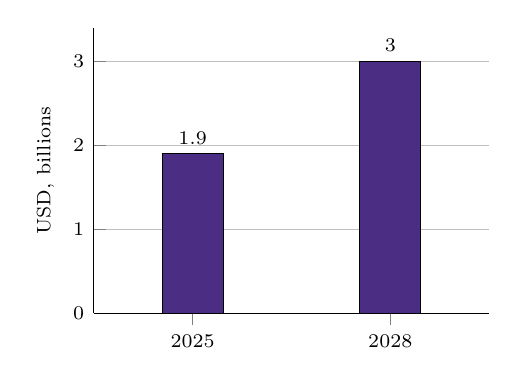
\begin{tikzpicture}
        \begin{axis}[
          ybar, bar width=22pt, width=6.6cm, height=5.2cm,
          symbolic x coords={2025,2028},
          xtick=data, ymin=0, ymax=3.4,
          ylabel={USD, billions}, ylabel style={font=\scriptsize},
          tick label style={font=\scriptsize},
          nodes near coords, nodes near coords style={font=\scriptsize},
          enlarge x limits=0.5,
          axis lines*=left, ymajorgrids]
          \addplot[fill=qViolet] coordinates {(2025,1.9) (2028,3.0)};
        \end{axis}
      \end{tikzpicture}
      \scriptsize Global quantum tech. market revenue \\ (QED-C, 2026 report)
    \end{column}
    \begin{column}{0.5\textwidth}
      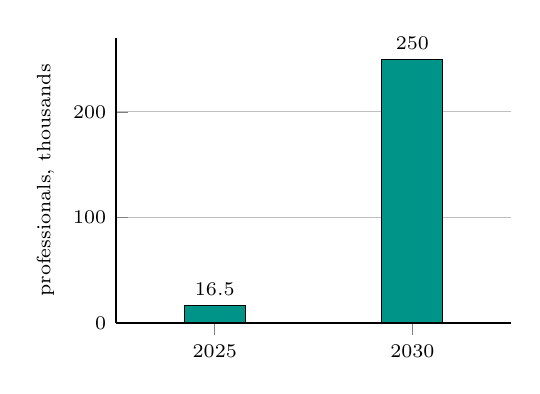
\begin{tikzpicture}
        \begin{axis}[
          ybar, bar width=22pt, width=6.6cm, height=5.2cm,
          symbolic x coords={2025,2030},
          xtick=data, ymin=0, ymax=270,
          ylabel={professionals, thousands}, ylabel style={font=\scriptsize},
          tick label style={font=\scriptsize},
          nodes near coords, nodes near coords style={font=\scriptsize},
          enlarge x limits=0.5,
          axis lines*=left, ymajorgrids]
          \addplot[fill=qCyan!70!black] coordinates {(2025,16.5) (2030,250)};
        \end{axis}
      \end{tikzpicture}
      \scriptsize Global quantum workforce, projected \\ (QED-C; The Quantum Insider)
    \end{column}
  \end{columns}
  \note{
    Numbers as of the QED-C "State of the Global Quantum Industry 2026"
    report and The Quantum Insider's 2026 workforce analysis -- cite these
    sources by name when presenting to administration, and mention this is
    a fast-moving snapshot (spring/summer 2026), worth re-checking before
    reusing this deck a year from now. Frame this slide as SUPPORTING
    context after the Pakistan-specific case, not the headline argument --
    it answers "is the rest of the world serious about this too?" once the
    room already knows the domestic policy and demand picture. Also worth
    mentioning: many quantum-software and research roles are remote-capable
    -- graduates trained in Pakistan can plausibly serve this global market
    without needing local hardware industry to exist first.
  }
\end{frame}

\begin{frame}{The skills gap is the argument}
  \begin{itemize}
    \item Analysis of thousands of quantum job postings worldwide: roughly
          \textbf{75\% of applicants lack the required skill profile}
    \item Demand spans \textbf{physics + computer science + electrical
          engineering} -- exactly the interdisciplinary mix universities
          are positioned to teach, and industry alone struggles to train
    \item \textbf{Low barrier to teach}: cloud access to real hardware
          (IBM Quantum, Amazon Braket, Azure Quantum) means \emph{no lab
          purchase required} to run a serious course
  \end{itemize}
  \note{
    This slide is aimed squarely at the administrators in the room. The
    "no lab purchase required" point is one of the strongest practical
    arguments you can make in a resource-constrained setting -- unlike
    standing up a wet-lab or fabrication course, a quantum computing course
    can start with free or low-cost cloud access to actual quantum hardware
    (IBM's Qiskit platform offers a free tier), open-source software
    (Qiskit, Cirq, PennyLane), and existing physics/CS faculty co-teaching.
    The skills-gap statistic is from EPJ Quantum Technology's analysis of
    ~3,600 job postings -- cite that provenance if pressed. Frame the ask
    explicitly: this is not "should we build a quantum lab," it's "should
    we teach the software/theory layer that students can practice on real
    cloud hardware for free" -- a much smaller institutional lift, and one
    HEC's curriculum has already scoped out for us.
  }
\end{frame}

\begin{frame}{What a first course could look like}
  \begin{enumerate}
    \item Linear algebra refresher through the lens of qubits \& gates
    \item Circuit model: single- and multi-qubit gates, measurement
    \item Core algorithms: Deutsch--Jozsa, Grover, Shor (conceptual)
    \item Hardware survey \& noise: NISQ reality, error correction basics
    \item Complexity theory: BQP and its neighbors
    \item Cryptographic impact: Shor's threat, post-quantum migration
    \item Capstone: run real circuits on cloud quantum hardware (Qiskit)
  \end{enumerate}
  \begin{center}\small
  \textit{Prerequisite: linear algebra + intro programming --- accessible
  to juniors, and a direct implementation of HEC's Quantum Computing
  specialization pathway}
  \end{center}
  \note{
    Keep this concrete and modest in scope -- a single semester, 3-credit
    elective, cross-listed between CS and Physics departments is a
    realistic, low-risk first step, not a whole new degree program (though
    IUB shows a full program is also a viable next step once demand is
    proven). If asked "who teaches it," note existing CS theory faculty
    (complexity/algorithms) and physics faculty (quantum mechanics) can
    co-teach with a semester of prep -- it does not require a brand-new
    hire on day one, which lowers the barrier to a pilot offering further.
    Explicitly note this maps onto HEC's already-published specialization
    pathway, so the institutional approval story is "implement the
    national standard," not "invent a new one."
  }
\end{frame}

\begin{frame}{Resources to start today}
  \begin{itemize}
    \item \textbf{Qiskit} (IBM) -- free, open-source, Python-based, runs on
          real cloud quantum hardware
    \item \textbf{IBM Quantum Learning}, \textbf{Amazon Braket tutorials},
          \textbf{Microsoft Azure Quantum} -- free courses and sandboxes
    \item \textbf{Nielsen \& Chuang}, \emph{Quantum Computation and Quantum
          Information} -- the field's standard textbook
    \item Pakistan-specific: \textbf{NCQC} (HEC), \textbf{CETQAP}
          outreach, and the annual \textbf{Quantum Computing Hackathon}
          (PIEAS/NILOP/NCP with CERN's OQI)
  \end{itemize}
  \note{
    Give students something to DO tonight, not just think about -- this is
    the single most effective way to convert curiosity into action right
    after a talk like this. Highlighting Pakistan-specific resources here
    matters: it signals this isn't only an import from Silicon Valley, a
    domestic ecosystem is already forming and students can plug into it
    directly. If time allows, consider live-demoing a 3-line Qiskit
    circuit on the free IBM Quantum cloud during Q\&A to make the "no lab
    purchase required" point viscerally real.
  }
\end{frame}

% ============================================================
\begin{frame}[standout]
  \small
  \textbf{Before this talk:} quantum = magic, replaces classical
  computers, breaks everything.

  \vspace{2mm}
  \textbf{Now:} quantum is \textbf{controlled interference}, it
  accelerates \textbf{specific} problems, and the bottleneck is
  \textbf{engineering}, not mystery.

  \vspace{5mm}
  \Large\textbf{Not magic. Not hype. Real physics, real limits, real
  jobs -- and, per HEC, already part of the answer.}

  \vspace{4mm}
  \normalsize Questions?
  \note{
    Closing line should land the whole talk's thesis in one sentence, and
    explicitly callback to the opening pop quiz: "remember the four
    options from the start? Now you can explain, technically, why option
    4 -- none of the above -- was correct, and what's half-true buried in
    each of the other three." Then open the floor. Anticipate: (1) "when
    will it actually be useful?" -- answer with the quantum-advantage
    timeline language from earlier (IBM targeting verified advantage by
    end of 2026, broader fault-tolerant systems widely estimated 2030s),
    stated as industry projection, not certainty; (2) "should students
    specialize in this now or is it too early?" -- answer: learn the
    FUNDAMENTALS (linear algebra, complexity theory) which are useful
    regardless of which hardware approach wins, rather than over-betting
    on one vendor's stack; (3) pushback from a skeptical faculty member
    about hype -- validate the skepticism (it's earned, the field has
    overclaimed before) while pointing back at the recap slide and the
    HEC-policy slide as the actual evidence-based position you're arguing
    for -- skepticism about specific claims and support for teaching the
    fundamentals are not in tension.
  }
\end{frame}

\end{document}
